% Options for packages loaded elsewhere
\PassOptionsToPackage{unicode}{hyperref}
\PassOptionsToPackage{hyphens}{url}
%
\documentclass[
]{book}
\usepackage{amsmath,amssymb}
\usepackage{lmodern}
\usepackage{ifxetex,ifluatex}
\ifnum 0\ifxetex 1\fi\ifluatex 1\fi=0 % if pdftex
  \usepackage[T1]{fontenc}
  \usepackage[utf8]{inputenc}
  \usepackage{textcomp} % provide euro and other symbols
\else % if luatex or xetex
  \usepackage{unicode-math}
  \defaultfontfeatures{Scale=MatchLowercase}
  \defaultfontfeatures[\rmfamily]{Ligatures=TeX,Scale=1}
\fi
% Use upquote if available, for straight quotes in verbatim environments
\IfFileExists{upquote.sty}{\usepackage{upquote}}{}
\IfFileExists{microtype.sty}{% use microtype if available
  \usepackage[]{microtype}
  \UseMicrotypeSet[protrusion]{basicmath} % disable protrusion for tt fonts
}{}
\makeatletter
\@ifundefined{KOMAClassName}{% if non-KOMA class
  \IfFileExists{parskip.sty}{%
    \usepackage{parskip}
  }{% else
    \setlength{\parindent}{0pt}
    \setlength{\parskip}{6pt plus 2pt minus 1pt}}
}{% if KOMA class
  \KOMAoptions{parskip=half}}
\makeatother
\usepackage{xcolor}
\IfFileExists{xurl.sty}{\usepackage{xurl}}{} % add URL line breaks if available
\IfFileExists{bookmark.sty}{\usepackage{bookmark}}{\usepackage{hyperref}}
\hypersetup{
  pdftitle={Grupo de Finanzas Sostenibles},
  pdfauthor={IngUAndes},
  hidelinks,
  pdfcreator={LaTeX via pandoc}}
\urlstyle{same} % disable monospaced font for URLs
\usepackage{longtable,booktabs,array}
\usepackage{calc} % for calculating minipage widths
% Correct order of tables after \paragraph or \subparagraph
\usepackage{etoolbox}
\makeatletter
\patchcmd\longtable{\par}{\if@noskipsec\mbox{}\fi\par}{}{}
\makeatother
% Allow footnotes in longtable head/foot
\IfFileExists{footnotehyper.sty}{\usepackage{footnotehyper}}{\usepackage{footnote}}
\makesavenoteenv{longtable}
\usepackage{graphicx}
\makeatletter
\def\maxwidth{\ifdim\Gin@nat@width>\linewidth\linewidth\else\Gin@nat@width\fi}
\def\maxheight{\ifdim\Gin@nat@height>\textheight\textheight\else\Gin@nat@height\fi}
\makeatother
% Scale images if necessary, so that they will not overflow the page
% margins by default, and it is still possible to overwrite the defaults
% using explicit options in \includegraphics[width, height, ...]{}
\setkeys{Gin}{width=\maxwidth,height=\maxheight,keepaspectratio}
% Set default figure placement to htbp
\makeatletter
\def\fps@figure{htbp}
\makeatother
\setlength{\emergencystretch}{3em} % prevent overfull lines
\providecommand{\tightlist}{%
  \setlength{\itemsep}{0pt}\setlength{\parskip}{0pt}}
\setcounter{secnumdepth}{5}
\usepackage{booktabs}
\usepackage{amsthm}
\makeatletter
\def\thm@space@setup{%
  \thm@preskip=8pt plus 2pt minus 4pt
  \thm@postskip=\thm@preskip
}
\makeatother
\ifluatex
  \usepackage{selnolig}  % disable illegal ligatures
\fi
\usepackage[]{natbib}
\bibliographystyle{apalike}

\title{Grupo de Finanzas Sostenibles}
\author{IngUAndes}
\date{Diciembre 2021, versión: 2021-12-14}

\begin{document}
\maketitle

{
\setcounter{tocdepth}{1}
\tableofcontents
}
\hypertarget{introducciuxf3n}{%
\chapter*{Introducción}\label{introducciuxf3n}}
\addcontentsline{toc}{chapter}{Introducción}

Las temáticas se relacionan con 3 Objetivos de trabajo:

\begin{itemize}
\tightlist
\item
  Descripción de un marco metodológico de trabajo
\item
  Aplicaciones: Energía (\protect\hyperlink{bib-amigo_two_2021}{Amigo, Cea-Echenique, and Feijoo, 2021}), Pensiones (\protect\hyperlink{bib-carlin_implementation_2015}{Carlin and Davies, 2015})
\item
  Validación experimental: (\protect\hyperlink{bib-dewan_estimating_2020}{Dewan and Neligh, 2020}), (\protect\hyperlink{bib-geller_gazer_2020}{Geller, Winn, Mahr, and Mirman, 2020})
\end{itemize}

\hypertarget{integrantes}{%
\section*{Integrantes}\label{integrantes}}
\addcontentsline{toc}{section}{Integrantes}

Tesista: José Tomás Pérez

Memoristas

\begin{itemize}
\tightlist
\item
  Vicente Muñoz
\item
  Ezequiel Ortíz
\end{itemize}

Ayudantes: Hernán Venegas

Investigador Responsable: Sebastián Cea

\hypertarget{planificaciuxf3n}{%
\section*{Planificación}\label{planificaciuxf3n}}
\addcontentsline{toc}{section}{Planificación}

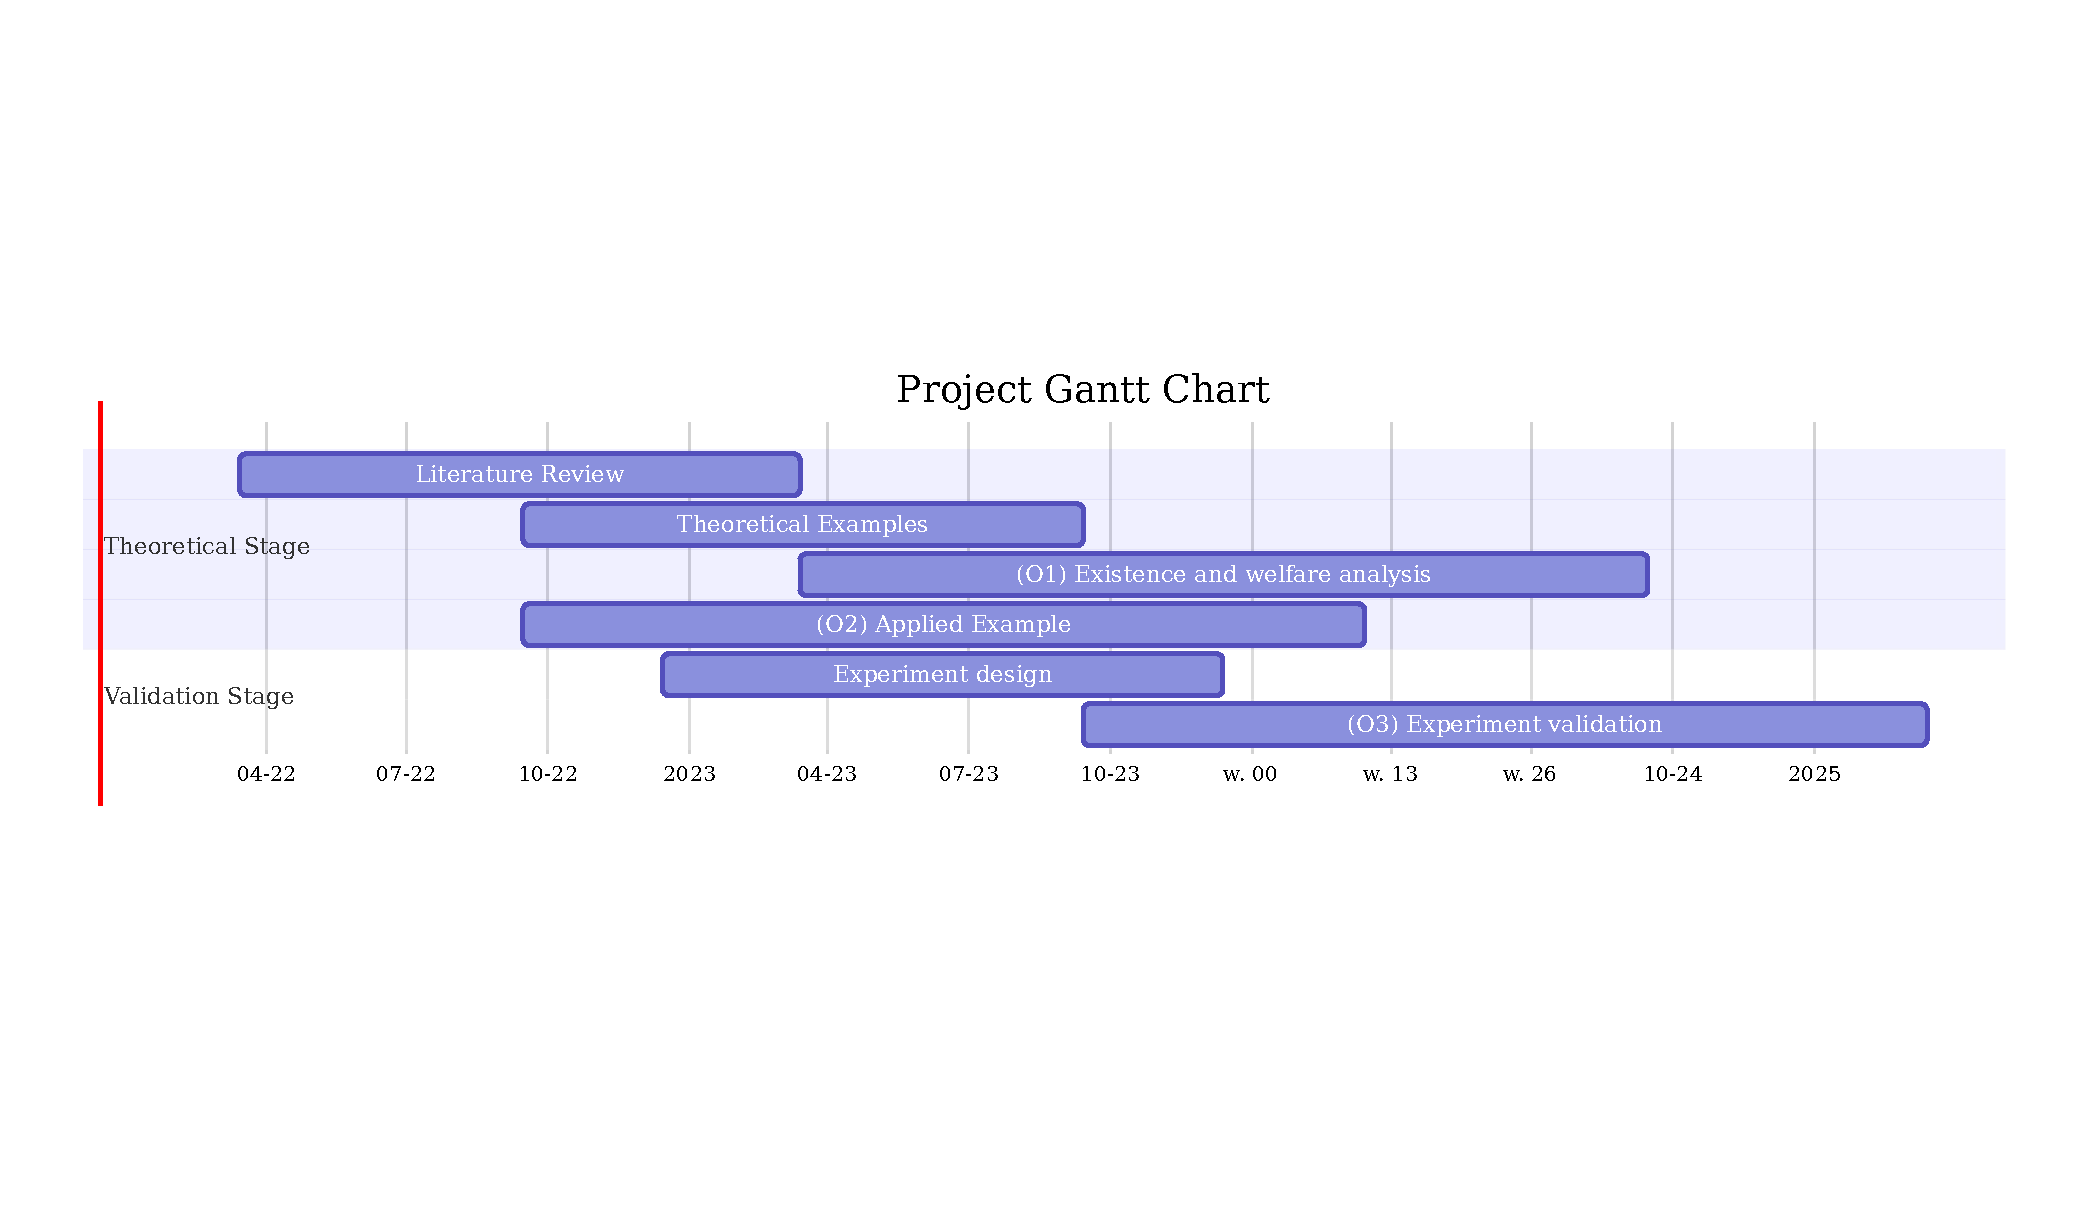
\includegraphics{bookdown-demo_files/figure-latex/unnamed-chunk-1-1.pdf}

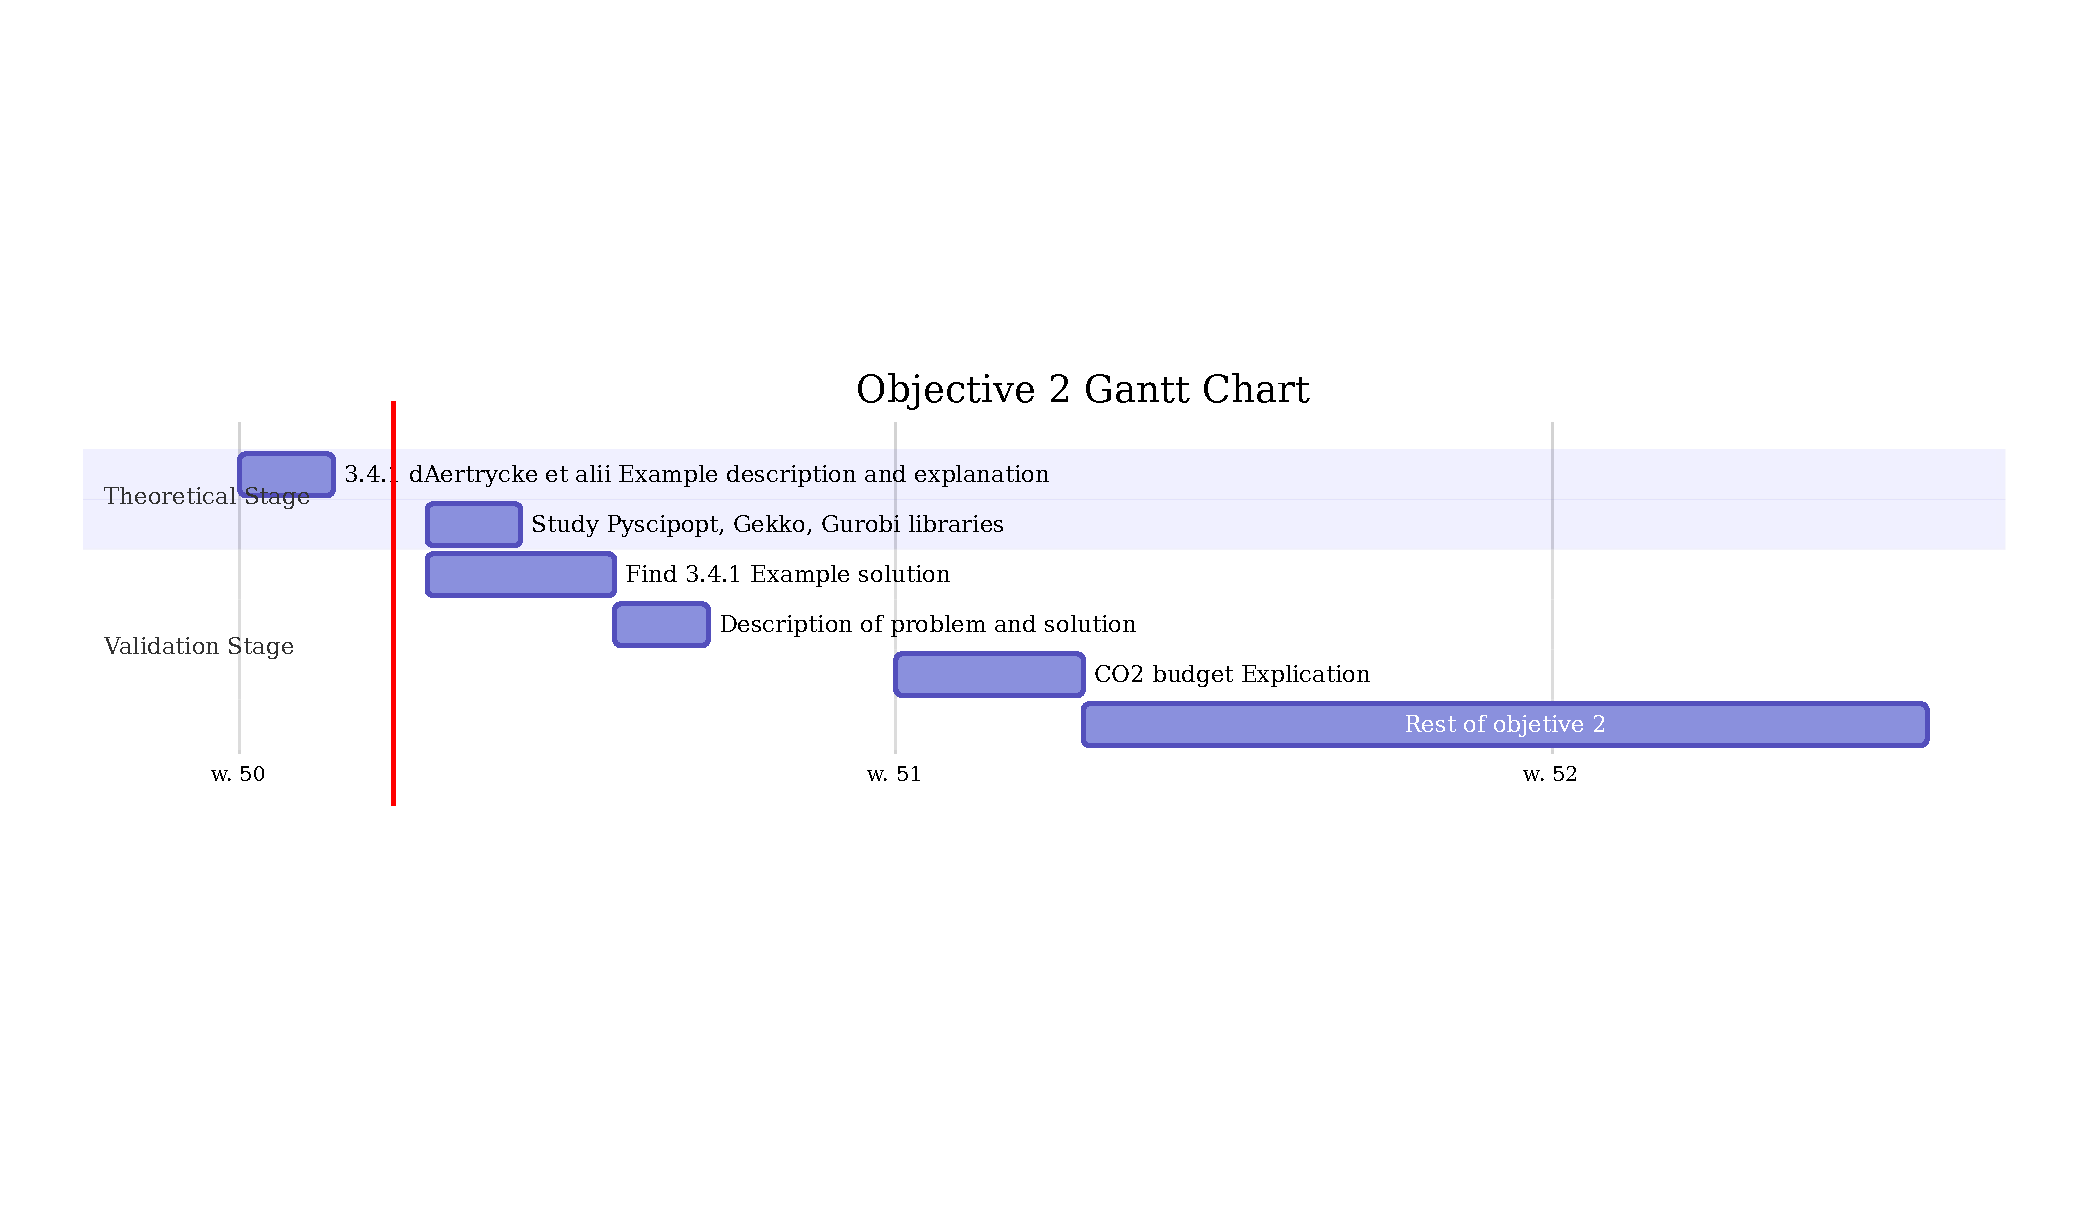
\includegraphics{bookdown-demo_files/figure-latex/unnamed-chunk-2-1.pdf}
\#\# Bibliografía base \{-\}

\protect\hyperlink{cite-amigo_two_2021}{Amigo, P., S. Cea-Echenique, and F.
Feijoo} (2021). ``A two stage cap-and-trade model
with allowance re-trading and capacity investment: The case of the
Chilean NDC targets''. En. In: \emph{Energy} 224, p.~120129. ISSN: 03605442.
DOI:
\href{https://doi.org/10.1016\%2Fj.energy.2021.120129}{10.1016/j.energy.2021.120129}.
URL:
\url{https://linkinghub.elsevier.com/retrieve/pii/S0360544221003789}
(visited on mar. 10, 2021).

\protect\hyperlink{cite-carlin_implementation_2015}{Carlin, B. I. and S.
Davies} (2015). \emph{The Implementation
of State Sponsored Retirement Plans}. En. SSRN Scholarly Paper ID
2589701. Rochester, NY: Social Science Research Network. DOI:
\href{https://doi.org/10.2139\%2Fssrn.2589701}{10.2139/ssrn.2589701}. URL:
\url{https://papers.ssrn.com/abstract=2589701}
(visited on nov. 02, 2020).

\protect\hyperlink{cite-dewan_estimating_2020}{Dewan, A. and N.
Neligh} (2020). ``Estimating information
cost functions in models of rational inattention''. En. In: \emph{Journal of
Economic Theory} 187, p.~105011. ISSN: 00220531. DOI:
\href{https://doi.org/10.1016\%2Fj.jet.2020.105011}{10.1016/j.jet.2020.105011}.
URL:
\url{https://linkinghub.elsevier.com/retrieve/pii/S002205311830396X}
(visited on mar. 23, 2021).

\protect\hyperlink{cite-geller_gazer_2020}{Geller, J., M. B. Winn, T. Mahr, et
al.} (2020). ``GazeR: A Package for Processing
Gaze Position and Pupil Size Data''. En. In: \emph{Behavior Research Methods}
52.5, pp.~2232-2255. ISSN: 1554-3528. DOI:
\href{https://doi.org/10.3758\%2Fs13428-020-01374-8}{10.3758/s13428-020-01374-8}.
URL:
\url{https://doi.org/10.3758/s13428-020-01374-8}
(visited on ene. 29, 2021).

\hypertarget{teoria}{%
\chapter{Teoría}\label{teoria}}

\hypertarget{atenciuxf3n-y-sofisticaciuxf3n-de-los-tomadores-de-decisiuxf3n}{%
\section{Atención y Sofisticación de los tomadores de decisión}\label{atenciuxf3n-y-sofisticaciuxf3n-de-los-tomadores-de-decisiuxf3n}}

\hypertarget{elecciones-discretas}{%
\subsection{Elecciones discretas}\label{elecciones-discretas}}

Ver propuesta \href{https://sebacea.github.io/drivers/DiscreteRI}{MathAmSud}

\hypertarget{seuxf1ales-de-informaciuxf3n-en-la-industria}{%
\section{Señales de información en la industria}\label{seuxf1ales-de-informaciuxf3n-en-la-industria}}

Descripción del cuestionario

\begin{itemize}
\tightlist
\item
  Descripción general del cuestionario
\end{itemize}

Se esta realizando un estudio que quiere conocer las estrategias de inversion que tienen diferentes agentes. En este se realiza una encuesta la cual tiene como objetivo conocer si los criterios de sostenibilidad son importantes para tomar una decisión sobre las inversiones que realiza el encuestado.

Por una parte, el encuestado tendra que responder preguntas generales sobre ``Inversiones Sostenibles''. Luego, tendrá que constestar otras preguntas las cuales estarán orientadas a la industria en la cual este se desempeña.

\begin{itemize}
\tightlist
\item
  Industrias involucradas
  El cuestionario también cuenta con una sección de preguntas las cuales estan orientadas a las diferentes industrias que estan involucradas con inversiones que poseen criterios de sostenibilidad.
\end{itemize}

Los encuestados pertenecen a las industrias de la banca, fondos de inversión, administradoras de fondos, generación eléctrica, consultoría, etc.

\hypertarget{aplicaciones}{%
\chapter{Aplicaciones}\label{aplicaciones}}

\hypertarget{energuxeda}{%
\section{Energía}\label{energuxeda}}

En el contexto de la energía, el medio ambiente es directamente afectado por la producción de esta. Para generar energía se necesita de la combustión de un material, del aprovechamiento mecánico de una energía natural externa u otros (nuclear). Y estos sistemas provocan, en distintos niveles y formas, efectos en el medio ambiente. Particualermente las termoeléctricas son concideradas como las que más emisiones de dióxido de carbono producen entre sus alternativas viables.Tambien, sandjan

\hypertarget{pensiones}{%
\section{Pensiones}\label{pensiones}}

Una aplicación para estudiar sistemas de pensiones es asumir una distribución de agentes atentos o sofisticados siguiendo el modelo de (\protect\hyperlink{bib-carlin_implementation_2015}{Carlin and Davies, 2015}).

\hypertarget{experimentos}{%
\chapter{Experimentos}\label{experimentos}}

\hypertarget{contenido-del-repositorio}{%
\section{Contenido del Repositorio}\label{contenido-del-repositorio}}

\begin{itemize}
\tightlist
\item
  Directorio Raíz contiene un documento integral de trabajo que genera una versión web accesible en \href{https://inguandes.github.io/FinSost/}{inguandes.github.io/FinSost/}
\item
  \href{docs}{\texttt{docs}} está expuesta públicamente como web
\item
  \href{code}{\texttt{code}} contiene códigos y plantillas de trabajo
\end{itemize}

  \bibliography{book.bib,packages.bib}

\end{document}
